% Main chapter title
\chapter{App Classification Models}
\label{ch:proposed}

% This is for the header on each page
\lhead{Chapter 5. \emph{App Classification Models}}
\thispagestyle{empty}
Classification is the technique to classify new observation on the basis of a set of data containing observations whose class is known \cite{wiki:xxx}. Classification is considered as an instance of supervised learning i.e. learning where training set of correctly identified observation is available. To build a classification model we need labelled data. We train classification model with using machine learning algorithm. Figure \ref{fig:appc1} shows the workflow of building the model. Once the model is trained, we feed new observation into classification model to classify them. Figure \ref{fig:appc2} shows the architecture of classifying the new observation using trained Model.
\begin{figure}[!h]
  \centering
  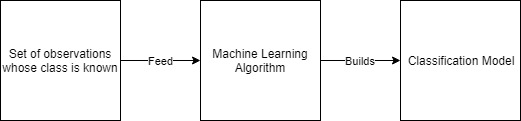
\includegraphics [scale=0.8] {appc1.jpg}
  \caption{Workflow of building a classification model.}
  \label{fig:appc1}
\end{figure}

\begin{figure}[!h]
  \centering
  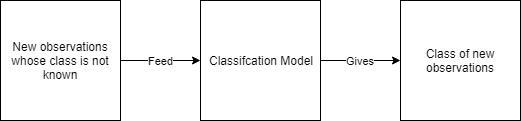
\includegraphics [scale=0.8] {appc2.jpg}
  \caption{Workflow of classifying the new observations.}
  \label{fig:appc2}
\end{figure}
To check the performance of model we have used confusion matrix \cite{wiki:xxx1}. A confusion matrix is a summary of prediction results on a classification problem. The number of correct and incorrect predictions are summarized with count values and broken down by each class. The confusion matrix shows the ways in which your classification model is confused when it makes predictions. It gives us insight not only into the errors being made by a classifier but more importantly the types of errors that are being made. A classification model is good if there is high value along the diagonal of confusion matrix. Table \ref{table:tab1} shows the general confusion matrix.\\
\begin{table}[!h]
\centering

\begin{tabular}{|l||l|l|}
\hline
\multirow{2}{4em}{Actual} & \multicolumn{2}{l|}{Predicted} \\ \cline{2-3} 
                  &    Benign      &    Malicious       \\ \hline
         Benign         &      TB     &     FM      \\ \hline
         Malicious          &     FB      &      TM     \\ \hline
\end{tabular}%

\caption{Confusion Matrix}
\label{table:tab1}
\end{table}\\
\textbf{Definition of the Terms: }
\begin{itemize}
    \item Benign (B): Observation is benign.
    \item Malicious (M): Observation is malicious.
    \item True Benign (TB): Observation is benign, and is predicted to be benign.
    \item False Malicious (FM): Observation is benign, but is predicted malicious.
    \item True Malicious (TM): Observation is malicious, and is predicted to be malicious.
    \item False Benign (FM): Observation is malicious, but is predicted benign.
\end{itemize}

We have collected the labelled data of 26000+ applications \cite{dataforclassmodel}.
Data set contains observations/traces of 25593 benign applications and 741 malicious applications. API calls has been used as the feature vector for application. Each application has 854 features. We have developed various classification models using machine learning techniques to classify new applications as benign or malicious. We have used following machine learning techniques:
\begin{enumerate}
    \item Logistic Regression
    \item Support Vector Machine
    \item Neural Network
    \item Random Forest
\end{enumerate} 

\section{Logistic Regression}
Logistic Regression is a classification technique which is is usually taken to apply to a binary dependent variable \cite{wiki:xxx2}. We have divided the data set into training set which is 80\% of the total data set and testing set which 20\% of the total data set. We have trained our model on the training set and have checked the performance of the model on test data. Model classifies 93.8\% of benign correctly and 83.4\% of malicious app correctly. Table \ref{table:tab2} shows the confusion matrix obtained from Logistic regression model. 
\begin{table}[!h]
\centering

\begin{tabular}{|l||l|l|}
\hline
\multirow{2}{4em}{Actual} & \multicolumn{2}{l|}{Predicted} \\ \cline{2-3} 
                  &    benign      &    malicious       \\ \hline
         benign         &      93.8     &    6.2       \\ \hline
        malicious          &     16.6      &      83.4     \\ \hline
\end{tabular}%
\caption{Confusion matrix for Logistic regression}
\label{table:tab2}
\end{table}
We have used this model to predict the class of applications which we have analyzed. Following application is classified as benign:
\begin{itemize}
    \item Budget Planner
    \item BHIM Making India Cashless
    \item System Certificate
    \item Tez: A new payment app by Google
    \item Google Calendar
\end{itemize}
Following application is classified as malicious:
\begin{itemize}
    \item Funnyys
    \item Omingo
    \item MMS Beline
    \item Laughtter
    \item Android Framework
\end{itemize}

\section{Support Vector Machine}
In machine learning, Support Vector Machine (SVM) is considered as supervised learning models associated with learning algorithms \cite{wiki:xxx3}. Here, we have used this model for classification. We have divided the data set into training set which is 80\% of the total data set and testing set which 20\% of the total data set. We have trained our model on the training set and have checked the performance of the model on test data. Model classifies 92.6\% of benign correctly and 78.7\% of malicious app correctly. Table \ref{table:tab3} shows the confusion matrix obtained from Support Vector Machine model.
\begin{table}[!h]
\centering

\begin{tabular}{|l||l|l|}
\hline
\multirow{2}{4em}{Actual} & \multicolumn{2}{l|}{Predicted} \\ \cline{2-3} 
                  &    benign      &    malicious       \\ \hline
         benign         &      92.6     &    7.4      \\ \hline
        malicious          &     21.3      &      78.7     \\ \hline
\end{tabular}%
\caption{Confusion matrix for Support Vector Machine}
\label{table:tab3}
\end{table}
We have used this model to predict the class of applications which we have analyzed. Following application is classified as benign:
\begin{itemize}
    \item Budget Planner
    \item Funnyys
    \item BHIM Making India Cashless
    \item System Certificate
    \item Tez: A new payment app by Google
    \item Google Calendar
\end{itemize}
Following application is classified as malicious:
\begin{itemize}
    \item Omingo
    \item MMS Beline
    \item Laughtter
    \item Android Framework
\end{itemize}

\section{Neural Network}
A Artificial Neural Network (ANN) or Neural Network (NN) is a machine learning technique which is inspired from the biological nervous system \cite{wiki:xxx4}. An ANN is based on a collection of connected units or nodes called artificial neurons which loosely model the neurons in a biological brain. We have divided the data set into training set which is 80\% of the total data set and testing set which 20\% of the total data set. We have trained our model on the training set and have checked the performance of the model on test data. Model classifies 96.3\% of benign correctly and 86.6\% of malicious app correctly. Table \ref{table:tab4} shows the confusion matrix obtained from Neural Network model.
\begin{table}[!h]
\centering

\begin{tabular}{|l||l|l|}
\hline
\multirow{2}{4em}{Actual} & \multicolumn{2}{l|}{Predicted} \\ \cline{2-3} 
                  &    benign      &    malicious       \\ \hline
         benign         &      96.3     &    3.7      \\ \hline
        malicious          &     13.4      &      86.6     \\ \hline
\end{tabular}%
\caption{Confusion matrix for Neural Network}
\label{table:tab4}
\end{table}
We have used this model to predict the class of applications which we have analyzed. Following application is classified as benign:
\begin{itemize}
    \item Budget Planner
    \item BHIM Making India Cashless
    \item Tez: A new payment app by Google
    \item Google Calendar
\end{itemize}
Following application is classified as malicious:
\begin{itemize}
    \item Funnyys
    \item Omingo
    \item System Certificate
    \item MMS Beline
    \item Laughtter
    \item Android Framework
\end{itemize}
\section{Random Forest}
Random Forest is a machine learning technique for classification, regression and other tasks \cite{wiki:xxx5}. It is made up of various decision trees \cite{wiki:xxx6}. We have used random forest for classification. We have divided the data set into training set which is 80\% of the total data set and testing set which 20\% of the total data set. We have trained our model on the training set and have checked the performance of the model on test data. Model classifies 97.2\% of benign correctly and 87.1\% of malicious app correctly. Table \ref{table:tab5} shows the confusion matrix obtained from Random Forest model. 
\begin{table}[!h]
\centering

\begin{tabular}{|l||l|l|}
\hline
\multirow{2}{4em}{Actual} & \multicolumn{2}{l|}{Predicted} \\ \cline{2-3} 
                  &    benign      &    malicious       \\ \hline
         benign         &      97.2     &    2.8     \\ \hline
        malicious          &     12.9      &      87.1     \\ \hline
\end{tabular}%
\caption{Confusion matrix for Random Forest}
\label{table:tab5}
\end{table}
We have used this model to predict the class of applications which we have analyzed. Following application is classified as benign:
\begin{itemize}
    \item \textbf{Benigin apps: }Budget Planner, BHIM Making India Cashless, Tez and Google Calendar.
    \item \textbf{Malicious apps: }Funnyys, Omingo, System Certificate, MMS Beline, Laughtter and Android Framework.
\end{itemize}

\section{Comparison}
We have used four classification algorithms namely Logistic Regression, Support Vector Machine (SVM), Neural Network, and Random Forest. Table \ref{table:com1} shows the comparison of accuracy of different algorithms.
\begin{table}[h!]
    \centering
    \begin{tabular}{|p{5cm}|p{4cm}|p{4cm}|}
      \hline
      \textbf{Algorithm} & \textbf{Accuracy of benign apps} & \textbf{Accuracy of malicious app}\\
      \hline
      \hline
      Logistic Regression & 93.8\% & 83.4\%   \\ \hline
      Support Vector Machine & 92.6\% & 78.7\%  \\ \hline
      Neural Network & 96.3\% & 86.6\% \\ \hline
      Random Forest & 97.2\% & 87.1\% \\ \hline
      
    \end{tabular}%
    \caption{Comparison of accuracy of different algorithms}
    \label{table:com1}
\end{table}
\\
Table \ref{table:com2} gives the information about whether app is identified as benign or malicious by various machine learning algorithms.
\begin{table}[h!]
    \centering
    \begin{tabular}{|p{3cm}|p{3cm}|p{3cm}|p{3cm}|p{3cm}|}
      \hline
      \textbf{Algorithm} & \textbf{Logistic Regression} & \textbf{SVM} & \textbf{Neural Network} & \textbf{Random Forest}\\
      \hline
      \hline
        Budget Planner&benign & benign & benign & benign  \\ \hline
        BHIM & benign & benign & benign & benign  \\ \hline
        Funnyys & malicious & benign & malicious & malicious  \\ \hline
        Omingo & malicious & malicious & malicious & malicious  \\ \hline
        System Certificate & benign & benign & malicious & malicious  \\ \hline
        Tez & benign & benign & benign & benign  \\ \hline
        MMS Beline & malicious & malicious & malicious & malicious  \\ \hline
        Google Calendar & benign & benign & benign & benign  \\ \hline  
        Laughtter & malicious & malicious & malicious & malicious  \\ \hline
        Android Framework & malicious & malicious & malicious & malicious  \\ \hline
    \end{tabular}%
    \caption{Categorization of apps into benign and malicious by various algorithm}
    \label{table:com2}
\end{table}